\documentclass[review]{elsarticle}

\usepackage{lineno,hyperref}
\modulolinenumbers[5]

\journal{Journal of \LaTeX\ Templates}

%%%%%%%%%%%%%%%%%%%%%%%
%% Elsevier bibliography styles
%%%%%%%%%%%%%%%%%%%%%%%
%% To change the style, put a % in front of the second line of the current style and
%% remove the % from the second line of the style you would like to use.
%%%%%%%%%%%%%%%%%%%%%%%

%% Numbered
%\bibliographystyle{model1-num-names}

%% Numbered without titles
%\bibliographystyle{model1a-num-names}

%% Harvard
%\bibliographystyle{model2-names.bst}\biboptions{authoryear}

%% Vancouver numbered
%\usepackage{numcompress}\bibliographystyle{model3-num-names}

%% Vancouver name/year
%\usepackage{numcompress}\bibliographystyle{model4-names}\biboptions{authoryear}

%% APA style
%\bibliographystyle{model5-names}\biboptions{authoryear}

%% AMA style
%\usepackage{numcompress}\bibliographystyle{model6-num-names}

%% `Elsevier LaTeX' style
\bibliographystyle{elsarticle-num}
%%%%%%%%%%%%%%%%%%%%%%%

\begin{document}

\begin{frontmatter}

\title{HPS calorimeter performances}

%% Group authors per affiliation:
\author{HPS collaboration}

%% or include affiliations in footnotes:
\author[mymainaddress,mysecondaryaddress]{Elsevier Inc}
\ead[url]{www.elsevier.com}

\author[mysecondaryaddress]{Global Customer Service\corref{mycorrespondingauthor}}
\cortext[mycorrespondingauthor]{Corresponding author}
\ead{support@elsevier.com}

\address[mymainaddress]{1600 John F Kennedy Boulevard, Philadelphia}
\address[mysecondaryaddress]{360 Park Avenue South, New York}

\begin{abstract}
The Heavy Photon Search experiement (HPS) aims to discover a new particle 
called heavy photon, that is the equivalent of the photon of the Standard 
Model for dark matter. It is detectable through its mixing with the 
standard photon. HPS is installed in the Hall B of Jefferson Laboratory, 
Virginia, United States of America. After a test run in 2012 and an 
engineering run in 2014, a first run was performed to acquire data. This 
paper presents the performances of one of the two detectors of the
experiment: the electromagnetic calorimeter (ECal).
\end{abstract}

\begin{keyword}
heavy photon, calorimeter, CLAS12, CLAS, Jefferson Laboratory, JLab
\MSC[2010] 00-01\sep  99-00
\end{keyword}

\end{frontmatter}

\linenumbers

\section{Introduction}

The heavy photon, also known as A' or dark photon, is a gauge boson that 
could be the equivalent of the ordinary matter photon for dark matter by 
being its electromagnetic force carrier. Heavy photons have been 
envisionned by numerous beyond Standard Model theories \cite{REssig}. It 
is also a good candidate to explain some astrophysical anomalies 
\cite{OAdriani-MAguilar}. The dark photon, that would interact with 
particles of the hidden sector, would mix with the ordinary photon through 
kinetic mixing \cite{} (add ref). It induces their weak 
coupling to electrons, $\epsilon$e, they can thus be radiated in electron 
scattering and consequently decay into electron-positron pairs. If the 
coupling is large enough, the resonance can be observed above the QED 
trident background, while if it is small enough, heavy photons travel 
detectable distances before decaying. The HPS experiment is designed to 
exploit both signatures. It will benefit of the full duty cycle of the 
electron beam available at JLab in Hall~B to cover two areas depending on 
the heavy photon mass and the strength of its coupling. To cover the 
largest area possible, three runs are planned with the following beam 
energy: 1.1 GeV, 2.2 GeV and 6.6 GeV and a luminosity comprised between 
200~nA and 500~nA. The silicon microstrip vertex tracker and the 
PbWO$_{4}$ electromagnetic calorimeter placed as close as possible of the 
0.15\%~-~0.25\%~X0 tungstene target will then allow the HPS experiment to 
be sensitive to heavy photons in the mass range of 20~MeV/c$^2$ to 
1000~MeV/c$^2$ (see fig. \ref{intro:covereddomain}). 

\nopagebreak
\begin{figure}[htb]
  \begin{center}
     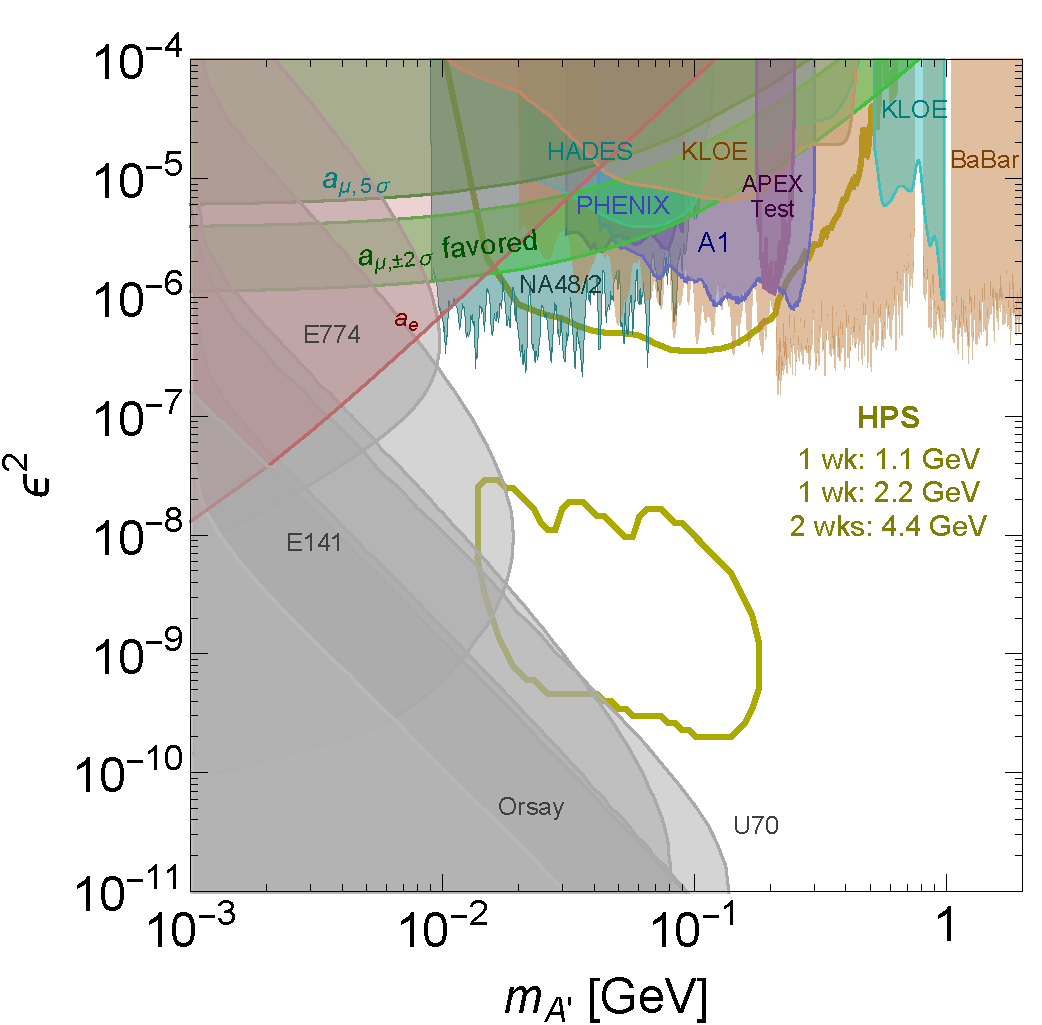
\includegraphics[angle=0, width=0.6\textwidth]
                           {A-visible-HPS-official-6-2015.pdf}
    \caption{Coupling factor as a function of the mass of the heavy 
     photon. In light green the area covered by the HPS experiment.}
    \label{intro:covereddomain}
  \end{center}
\end{figure}


The experiment is installed in the Hall-B at Jefferson Lab. In addition to 
the detectors, an analyzing magnet allows to determine the charge and 
momentum of the particles. Two magnets installed downstream and upstream 
of the target complet the setup to ensure that the beam reaches the beam dump 
(see fig. \ref{intro:HPSScheme}).

\nopagebreak
\begin{figure}[htb]
  \begin{center}
     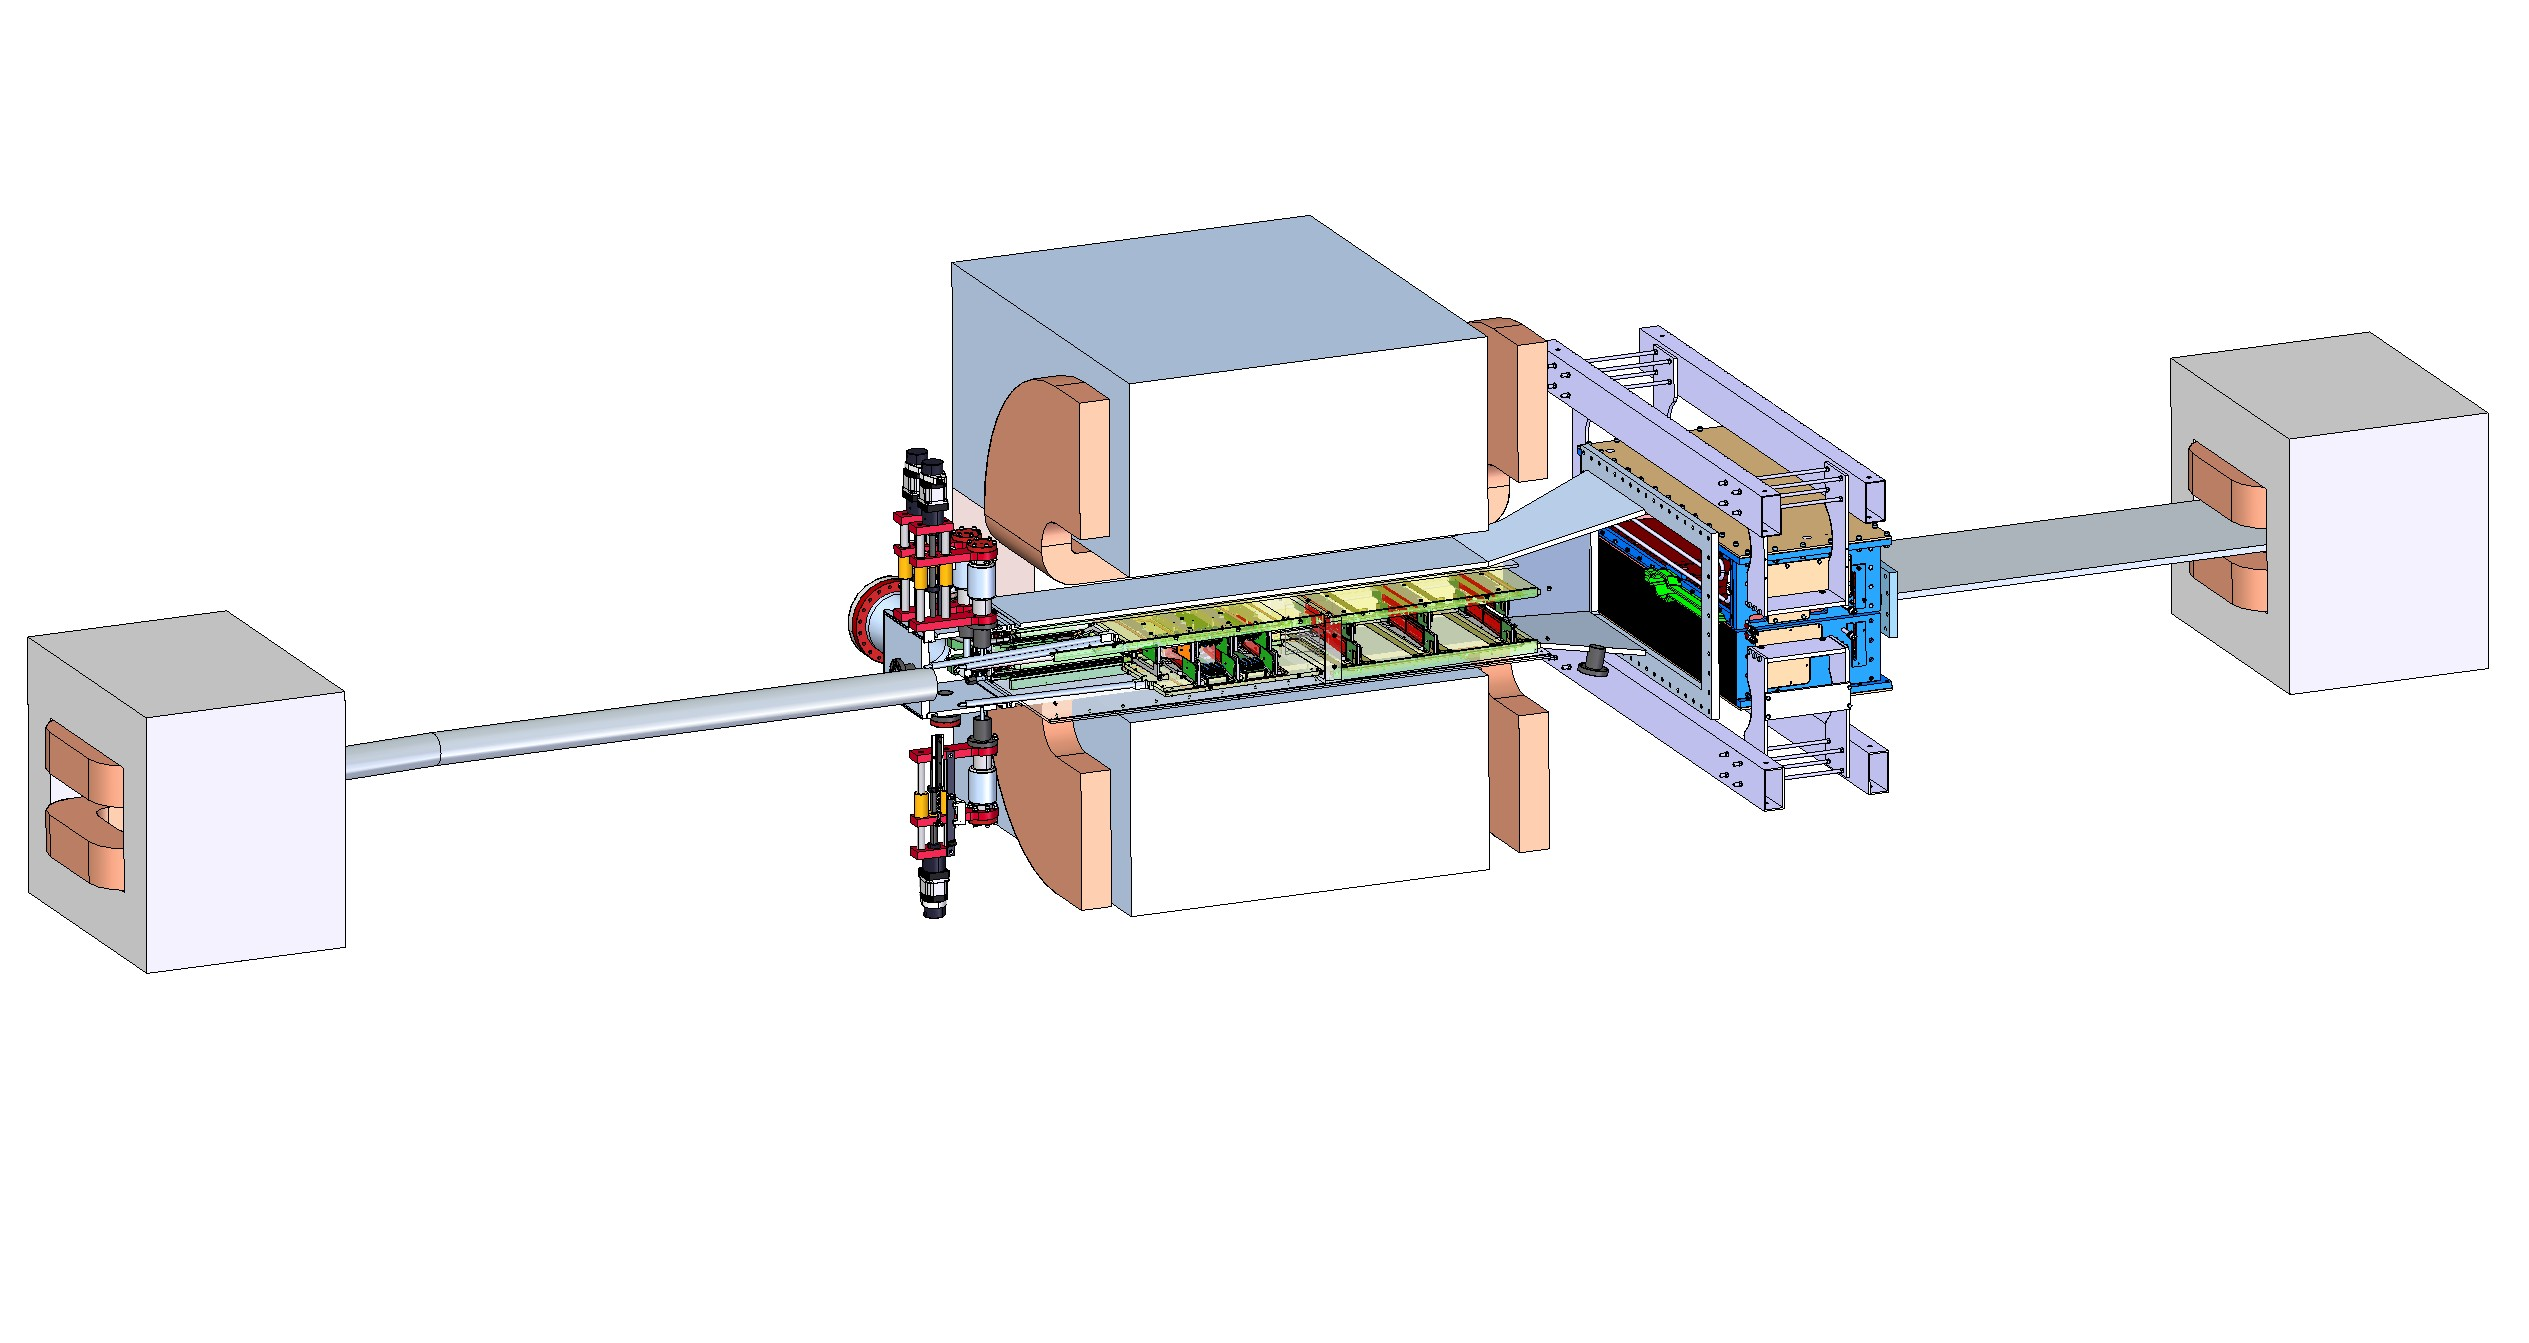
\includegraphics[angle=0, width=0.9\textwidth]{HPS_pic.jpg}
    \caption{Schematic layout of the HPS experiment.}
    \label{intro:HPSScheme}
  \end{center}
\end{figure}


A test run was performed in May 2012 with a partial detector setup, which 
results can be found in \cite{HPSTestRun}. We detail here the performances 
of the final calorimeter during the engineering runs of Winter 2014 and 
spring 2015. The paper is organised as follow: we first presents the 
calorimeter layout as well as the modifications made to the calorimeter 
after the test run. The two following sections are about the time and 
energy calibration of the detector. Eventually, a presentation of the 
performance of the LED system used to monitor the crystals is given.

{(\bf should we describe/discuss trigger? fADC? TDC? and pre-amplifiers?)}

\section{Calorimeter layout}

The ECal is built in two separate halves that are mirror reflections of 
one another about the plane of the nominal electron beam to avoid 
interfering with a horizontal 15 mrad zone of very high flux. This zone is 
due to the dipole magnet that spreads the degraded beam on a plane. As 
shown in Figure \ref{Calo}, the 221 modules in each half, supported by 
aluminum support frames, are arranged in rectangular formation with five 
layers and 46 crystals/layer except for the layer closest to the beam 
where nine modules were removed to allow a larger opening for the outgoing 
electron and photon beams. 

Each crystal (see fig. \ref{Crys}) is a 160~mm long tapered parallepiped 
with a front (rear) face of 13.3$\times$13.3~mm$^ {2}$ 
(16$\times$16~mm$^{2}$). The crystals were previously used for the inner 
calorimeter of CLAS, they have been equipped with 10$\times$10~mm$^ {2}$ 
Large Area APD (LAAPD-Hamamatsu XXX) ({\bf add product ref}). The new 
LAAPD allows to collect more light, those increasing the signal over noise 
ratio leading to a lower energy threshold and an improved energy 
resolution. The signal from the APDs is first sent to a preamplifier
converting current-to-voltage (0.62 V/pC) which was designed to have low 
impedance and low noise ({\bf add diagram and maybe more details or ref?}). 
Finally, 2/3 of the signal is sent to the fADC({\bf ref?}), the other part 
being sent to a TDC.

The gain of the APDs was chosen to be the best compromise between high gain 
and low dark current ({\bf Do we have values/figures to motivate the 
choice then?}). The voltage of each APD group is then selected so that the 
gain is near 150 for each APD. ({\bf add the equation and values to get MeV 
to V conversion}) The gain of the preamplifier was adjusted to 0.62 V/pC to 
ensure that maximum energy deposition, estimated to be 4 GeV in a single 
crystal, would not saturate the fADC.

In front of the crystals are installed LED placed in plastic holders 
to send iin the crystal either blue or red light. Their principaly used
to check the functionning of the crystal and the amplification chain. In
the future studies will be carried to study how they can help crystals to
recover from radiation dammage.

\begin{figure}[ht!]
\centering
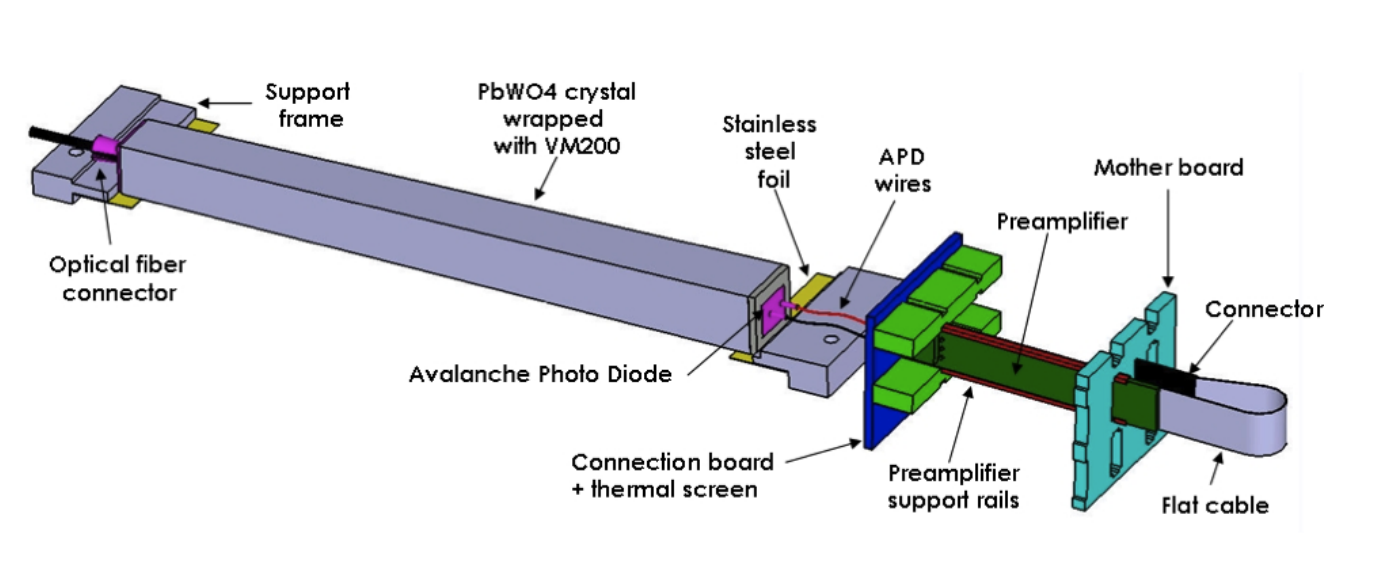
\includegraphics[width=0.70\textwidth]{CrystalView.png}
\caption{A schematic view of an ECal module.}
\label{Crys}
\end{figure}


To stabilize the crystal light yield and the operation of the APDs, each half of the calorimeter is enclosed in a temperature 
controlled box ($<$1$^{\circ}$C stability and $<$4$^{\circ}$C uniformity
{\bf Do we need a chart of Temp to illustrate?}). This is 
especially important because of the power drawn by the 
preamplifiers, 0.11~W each. The operating voltage of the preamplifiers ($\pm$5~V), 
the bias voltage of the APDs ($\approx$~400~V), and the read out channels from the 
APDs are supplied by four new printed circuit boards mounted on the backplane penetrating the enclosure. They were completely redesigned after the 2012 
test run and a very careful attention was brought to avoid cross-talks 
between channels. Each half of the ECal is divided into 14 bias voltage 
groups. Indeed, APDs are inherently produced with different gain to voltage
characteristics. The cautious selection of APD groups, their matching with 
the preamplifiers and adjusting the high voltage lead to a total gain 
uniformity of about 2\% ({\bf confirmed by calibration data?}), which 
highly simplify our trigger setup.

During the run, both halves were held in place by vertical threaded rods 
attached to rails above the analyzing magnet. Surveys carried out before 
the runs have shown that the distance between the target and the front 
face of the crystals is on average XX~cm. The gap between the two halves 
being XX~cm, corresponding to a minimum incident angle of XX mrad. 
({\bf numbers to update}) The surveys have also shown that the initial
positions of the two halves can be easily retrived within 0.3~mm after
moving the detector out to access the SVT or do maintenance work.

\begin{figure}[ht!]
\centering
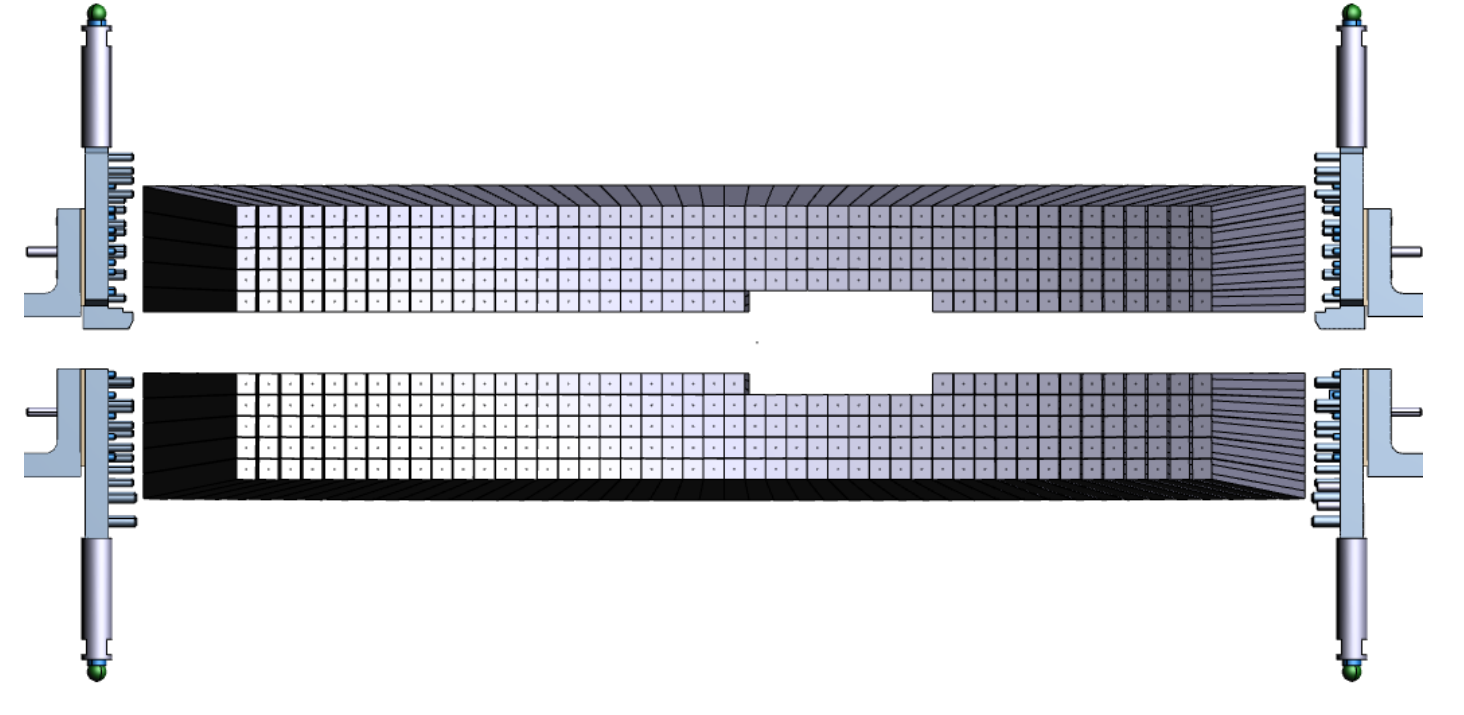
\includegraphics[width=1.00\textwidth]{ViewCalo.png}
\caption{Schematic view of an ECal module.}
\label{Calo}
\end{figure}




\section{Time calibration}

The time calibration is a key element for our experiment as our trigger is 
based on the measurement coincidences in the two halves of the calorimeter. 
A good time precision reduces the occurance of accidental coincidences which 
we want to minimize. The time of a cluster is set from the crystal with the 
highest energy in this cluster. This signal, sampled at 250~MHz by a fADC, is 
fitted with a 3-pole function (TODO: need formula here) for which parameter
X is directly the time of the hit. We show in this part how we determined the 
time offsets for each channel and how time walk and resolution vary as a 
function of the energy. (TODO make sure the last statement is correct)

The calibration of the time offsets is done in two steps. The first one relies 
on the accelerator radiofrequency (RF) signals, which indicate the structure of
bunches of the beam and the second one, on correlated cluster pairs.
(TODO I think it needs a little more explanation here)

\subsection{Offsets}

This correction relies on the fact that the CEBAF beam enters Hall B at 
499~MHz and the accelerator provides a signal every 80 bunches that we
measure on a channel of our fADC boards in the exact same conditions than
our experimental signals. The precision at which the accelerator signal is 
measured has been determined to be 24~ps. This signal being sampled every 80 
bunches the time difference between the RF signal and a crystal is expected 
to present peaks spaced by 2~ns as one can see Figure~\ref{RF}. One of these 
peak should be at 0 allowing for a first time calibration {\it modulo} 2~ns.

\begin{figure}[ht!]
\centering
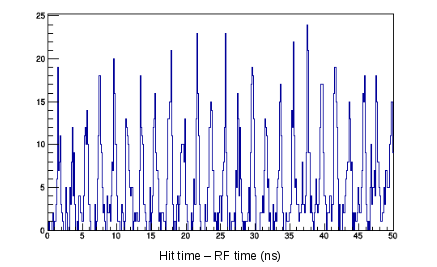
\includegraphics[width=0.70\textwidth]{crystalSpectra.png}
\caption{Difference in time between a single crystal hit and the RF time.}
\label{RF}
\end{figure}

To evaluate offsets larger than 2~ns, we use the time difference between 
clusters from M$\o$ellers and trident production \footnote{to be discussed}. 
Correlated cluster candidates must have an energy sum close to the beam energy, 
an energy difference less than 200~MeV and occur in the same 40~ns time window. 
The time difference between these pairs is then obtained for each crystal. 
(TODO clarify, there must be two crystals involved each time) The 
resultant distributions provide again a 2~ns interval patern as seen in 
Figure \ref{LargeOffset}, the largest peak indicating the correct offset.

\begin{figure}[ht!]
\centering
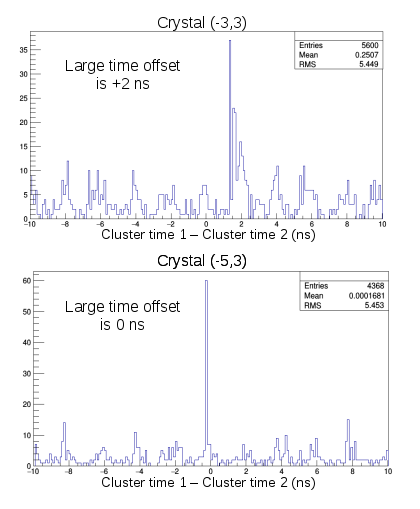
\includegraphics[width=0.70\textwidth]{pairsProcedure.png}
\caption{Time difference between the seed hit of two correlated clusters after 
RF calibration. The top and bottom plots show events for two different seed hit crystals.}
\label{LargeOffset}
\end{figure}

The total time offset for each crystal can finally be obtained as the sum of 
the two methods and are presented in Figure \ref{TimeOffset}). We notice that a
particular group has -4 ns time offsets, it corresponds to a group of channels 
using a shorter readout cable from the ECal to the FADC.


\begin{figure}[ht!]
\centering
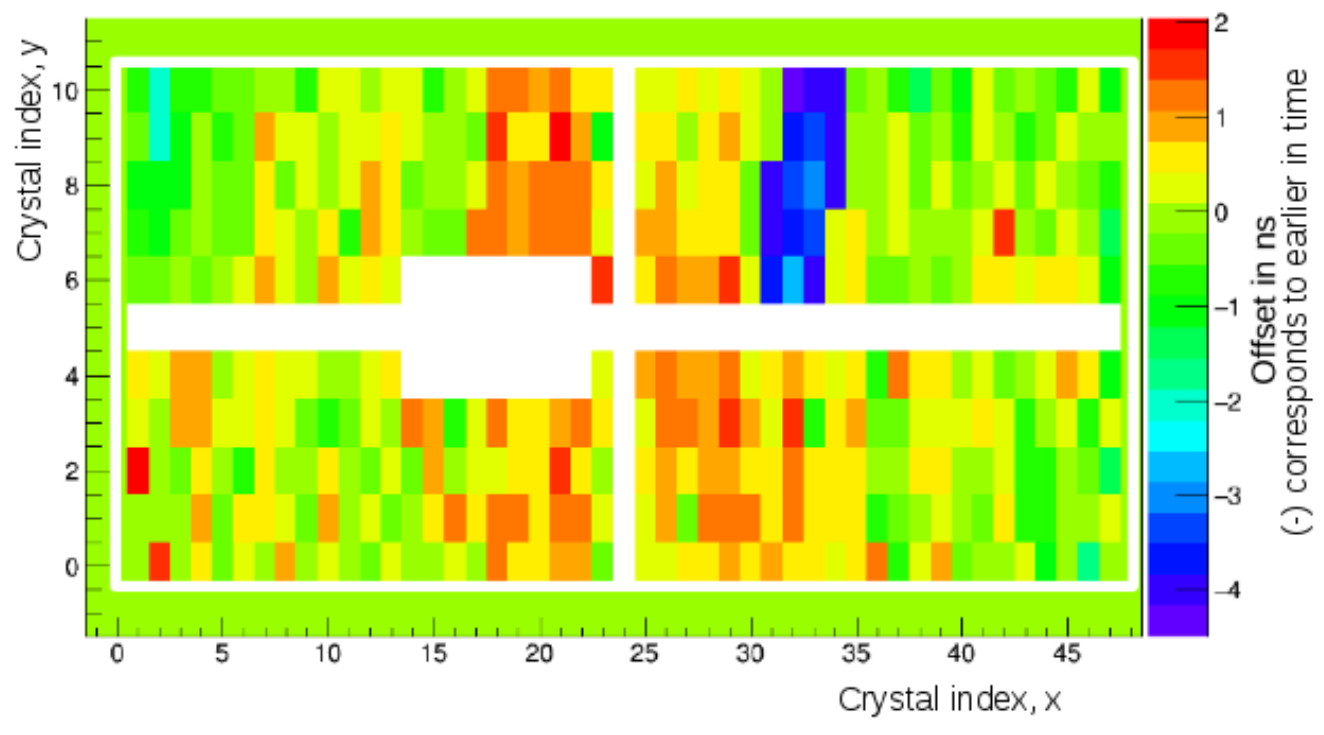
\includegraphics[width=0.70\textwidth]{TimeOffset.png}
\caption{Individual time offsets for each crystal.}
\label{TimeOffset}
\end{figure}

\subsection{Energy dependent time walk}

The time offsets can be energy dependent if there is time walk (TODO I do not 
think this is the proper term), we studied the difference of time between hits 
in a single cluster versus the highest energy hit as a function of energy. The 
results are fitted by an decreasing exponential and a second order polynomial,
as shown in Figure~\ref{TimeWalk}, and be corrected.
(TODO I think this is mainly due to the form of the signal, I am not sure what 
time walk means otherwise? That definitely need more discussion)

\begin{figure}[ht!]
\centering
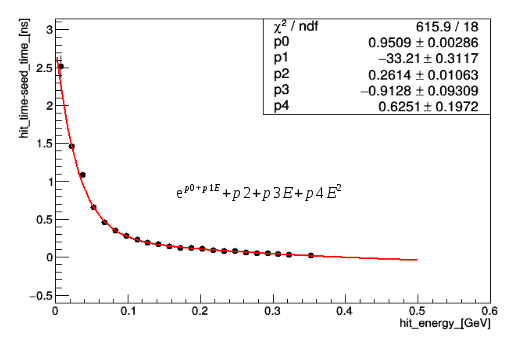
\includegraphics[width=0.70\textwidth]{twalk.png}
\caption{Time walk correction for clusters where the seed hit energy is greater than 400~MeV.}
\label{TimeWalk}
\end{figure}

%I did not understand the argument
%From this result, one can see that the time walk correction is small above 
%150~MeV, hence time walk correction needs to be applied only between crystals 
%of the same cluster using the seed hit as a reference.

Finally, the time resolution as a function of the energy can be plotted from 
the width of the time cluster time coincidences shown in Figure \ref{TresoVSTime}. 
We find this time resolution to be:

\begin{equation}
\textrm{Time resolution}= \frac{0.052}{E~(\textrm{GeV})} + 0.2044~\textrm{ns}.
\label{eq}
\end{equation}


\begin{figure}[ht!]
\centering
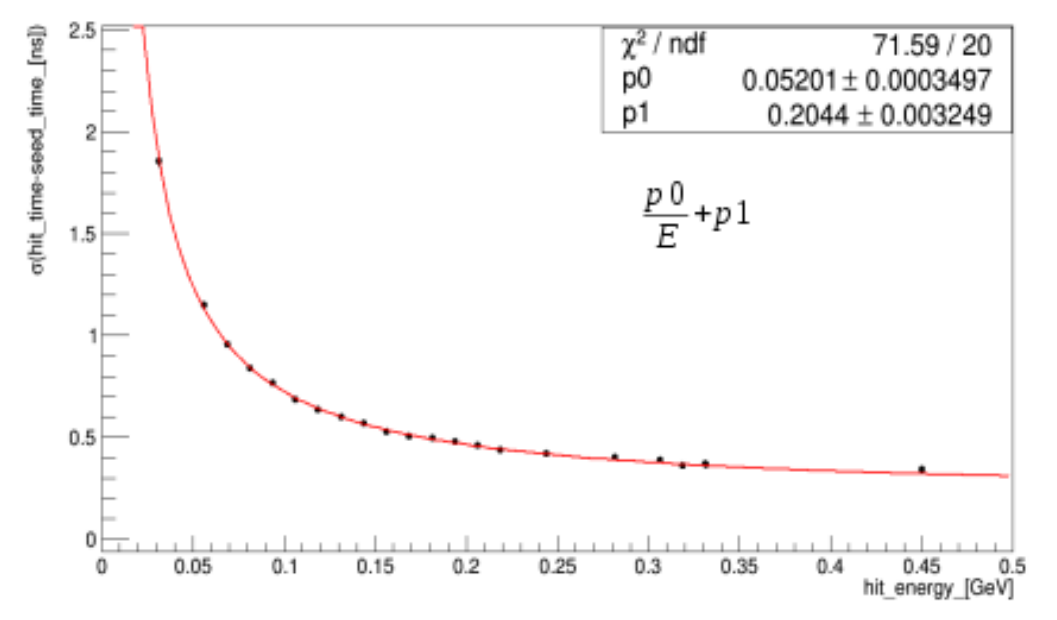
\includegraphics[width=0.70\textwidth]{TimeResolution.png}
\caption{Individual crystal time resolution as a function of energy.}
\label{TresoVSTime}
\end{figure}

The time resolution obtained shows the good performances of HPS electromagnetic 
calorimeter and a good capability to recover a time
precision well below the initial sampling size (i.e. 4 ns).
TODO Last line make me think we should show some signal fits

\section{Energy calibration}
(Holly)

We should probably wait for the results with the new ECal geometry 
implementation. But, almost everything can be written and the plots will be 
added at the last moment.

Describe the method used to determine the energy calibrations: 
cosmics 
short description of the clustering algorithm: seed+crystals around+what we do with piled up clusters.
Description of the events used for the calibration.
Then results obtained with the method. Energy resolution as a function of the energy and position. 

\section{Trigger performance?}

\section{LED system}
(Andrea)

We present here, the performances of the LED system. 

\section{Conclusions}

Main points:
 - Good time resolution with large sampling
 - Importance (or not?) of crystal spacing for energy resolution ???
 - Stability of the LED system

\section*{References}

%\bibitem{REssig} R. Essig, J. A. Jaros, W. Wester, P. H. Adrian, S. Andreas, et al. (Report of the Community Summer Study 2013 (Snowmass) Intensity Frontier New, Light, Weakly-Coupled Particles subgroup), Dark Sectors and New, Light, WeaklyCoupled Particles, 2013. URL 〈http://arxiv.org/abs/arXiv:1311.0029〉.

%\bibitem{OAdriani} O. Adriani, et al., PAMELA Collaboration, Nature 458 (2009) 607.
%\bibitem{MAckermann} M. Ackermann, et al., Fermi LAT Collaboration, Physical Review Letters 108 (2012) 011103.
%\bibitem{MAguilar} M. Aguilar, et al., AMS Collaboration, Physical Review Letters 110 (2013) 141102.
%\bibitem{HPSTestRun} M. Battaglieri, et al., \textit{The Heavy Photon Search Test Detector}, Nucl. Instrum. Meth. A777 (2014) 91-101

\bibliography{mybibfile}

\end{document}
